\documentclass[10pt,twocolumn,letterpaper]{article}

\usepackage{cvpr}
\usepackage{times}
\usepackage{epsfig}
\usepackage{graphicx}
\usepackage{amsmath}
\usepackage{amssymb}

% Include other packages here, before hyperref.

% If you comment hyperref and then uncomment it, you should delete
% egpaper.aux before re-running latex.  (Or just hit 'q' on the first latex
% run, let it finish, and you should be clear).
\usepackage[breaklinks=true,bookmarks=false]{hyperref}

\cvprfinalcopy % *** Uncomment this line for the final submission

\def\cvprPaperID{****} % *** Enter the CVPR Paper ID here
\def\httilde{\mbox{\tt\raisebox{-.5ex}{\symbol{153}}}}

% Pages are numbered in submission mode, and unnumbered in camera-ready
%\ifcvprfinal\pagestyle{empty}\fi
\setcounter{page}{1}
\begin{document}

%%%%%%%%% TITLE
\title{Pedestrian Detection Using Correlated Lidar and Image Data}

\author{Samuel Rohrer\\
University of Michigan\\
{\tt\small rohrer@umich.edu}
% For a paper whose authors are all at the same institution,
% omit the following lines up until the closing ``}''.
% Additional authors and addresses can be added with ``\and'',
% just like the second author.
% To save space, use either the email address or home page, not both
\and
Ian Lin\\
University of Michigan\\
{\tt\small tiannis@umich.edu}
}

\maketitle
%\thispagestyle{empty}

%%%%%%%%% ABSTRACT
\begin{abstract}
  Recent progress in software and hardware systems will lead to an increase in
  daily interactions with robots and intelligent systems. As a result of this
  safety must be at the forefront of the design of autonomous systems,
  particularly autonomous cars. With this in mind we aim to create a pedestrian
  detection system based off of sensors commonly found on autonomous vehicles.
  We will use correlated Lidar and image data along with algorithms found in
  recent papers to perform pedestrian detection.

\end{abstract}

%%%%%%%%% BODY TEXT
\section{Introduction}

  As progress in software and hardware continues, it is expected that
  autonomous robotics and intelligent systems will begin to play an integral
  role in everyday life. Jobs that are physically demanding or unsafe can be
  replaced by robots and autonomous cars can greatly improve road safety and
  efficiency. In order for these intelligent systems to succeed, safety must
  be at the forefront of their design. Detection of obstacles is a very
  significant aspect of this concern, especially for autonomous cars which
  must detect not only other cars, but also road signs, traffic signals, and
  pedestrians. In particular, pedestrian detection is an ongoing research
  area within computer vision.

  The goal of this project is to detect pedestrians in a pre-existing dataset:
  the LIPD dataset provides correlated LIDAR data and image data. We aim to do
  this by identifying obstacles on the road, based on LIDAR data, and
  associating these obstacles to the image data through feature extraction.
  After feature extraction, we plan to use a trained classifier to determine
  if the obstacle is indeed a pedestrian in the road. We could extend this by
  training a more sophisticated classifier that has the ability to discern the
  difference between cars, pedestrians, and road signs.

%------------------------------------------------------------------------
\section{Previous Work}

  There has been a good deal of work in the area of pedestrian detection for
  mobile robotics. In most systems, the sensor subsystems operate independently
  of each other. In \cite{journal} the authors use Lidar to generate regions
  of interest, then use image analysis to determine the presence of a
  pedestrian. Some other sensors available on modern autonomous robotics
  platforms include: radar, ultrasound, camera sensors and Lidar (light
  detection and ranging). However, each of these sensors comes with their own
  inherent problems. Cameras can fail in low light situations, and Lidar can
  fail when objects are side by side at the same distance. Both can fail in poor
  weather, as Lidar can fail if rain or snow causes the light to be reflected
  too early and camera images can fail if the lens is obstructed by poor weather.

  In order to complete this project, we started with a data set \cite{dataset}.
  Some benefits of this dataset include: correlated Lidar and image data, and
  a classification dataset. The correlated datasets were composed of a forward
  facing camera (limited field of view relative to Lidar) and four Lidar scans
  all facing outwards at different angles. The classification dataset had both
  training and testing sets for the Lidar.


%------------------------------------------------------------------------
\section{Technical Work}

  We plan to use both the Lidar data and image data together to identify
  pedestrians on the road. With Lidar data, we can identify obstacles on the
  road and then analyze the corresponding images that potentially contain
  pedestrians. There has already been work done in the areas of correlating
  Lidar and single image data for the purpose of detecting pedestrians. Most
  of it follows the same approach that we are outlining and has had succes.
  For Lidar object detection, we decided to follow the pipeline outlined
  in \cite{journal}, and add stages for error correction and correlation with
  image data. The pipeline is as follows: segmentation, feature
  extraction, classification, error correction, and correlation with image data.

  \subsection{Lidar Segmentation}
  The pipeline begins with segmentation of the Lidar data
  to find the points where the directionality of the segment changes.
  According to \cite{conf} if it
  is a new segment then (1) holds true where $r_i$ is the
  distance to current point, $r_{i+1}$ is the distance to next point,
  $cos(\Delta \alpha)$ is the 3D angle between the two points, and $C_0$ is a
  constant to adjust for noise:
   \begin{equation} \sqrt{r_{i}^{2} + r_{i+1}^{2} - 2 r_{i} r_{i+1}
   cos(\Delta \alpha)} > thd \end{equation}
   \begin{equation} thd = C_0 + \sqrt{2(1-cos(\Delta \alpha} * min(r_i,
   r_{i+1}) \end{equation}

  For the purpose of this project any segment less than three points long was
  discarded before moving to feature extraction. This was performed for each
  Lidar scan in isolation of the other scans.

  \subsection{Feature Extraction}
  After separating the Lidar scan data into different segments we then
  performed feature extraction on the segments. We used 10 different features
  for each segment, based on \cite{journal}.

  \renewcommand{\arraystretch}{1.5}
  \begin{center}
    \begin{tabular}{ | p{1cm} | l | p{2.9cm} |}
      \hline
      Feature num & Formula & Description \\ \hline
      1 & $ np $ & number range points \\ \hline
      2 & $np*r_{min}$ & number of range points * minimum range distance \\ \hline
      3 & $\sqrt{ \Delta X^2 + \Delta Y^2} $ & RMS of segment width and height
      \\ \hline
      4 & $ \frac{1}{np}\sum_{n=1}^{np} || x_n - x_m|| $ & Mean average deviation
      from median ($x_m$) \\ \hline
      5 & $ \frac{1}{np}\sum_{n=1}^{np} (x_n - x_{lsq})^2 $ & Linearity -
      distance to the least squares line ($ x_{lsq}$) \\ \hline
      6 & $ \frac{1}{np}\sum_{n=1}^{np} (x_n - \mu_x)^2 $ & Second central
      moment (about mean $\mu_x$) \\ \hline
      7 & $ \frac{1}{np}\sum_{n=1}^{np} (x_n - \mu_x)^3 $ & Third central
      moment (about mean $\mu_x$) \\ \hline
      8 & $ \frac{1}{np}\sum_{n=1}^{np} (x_n - \mu_x)^4 $ & Fourth central
      moment (about mean $\mu_x$) \\ \hline
      9 & $ \sum_{n=1}^{np} ||x_n - x_{n-1}|| $ & Segment length (norm distance
      between points) \\ \hline
      10 & $ \sigma(ft9) $ & Standard deviation of
      segment length (norm distance between points) \\ \hline
    \end{tabular}
  \end{center}

  These features describe the distribution of segment points and were all able to
  be computed quickly and robustly for all segments greater than three points long.

  \subsection{Classification}
  For classification we used training data from \cite{dataset} to train a Python
  SkLearn DecisionTreeClassifier \cite{sklearn}. The training data consisted of
  pre-segmented lidar scans that were very clean and well segmented. The lidar
  scans were split between segments with pedestrians and segments without
  pedestrians. A similar set of test data was also provided and our classifier
  achieved an accuracy of 88\%.



%------------------------------------------------------------------------
\section{Experimental Results}
  We ran our pipeline on raw lidar scans correlated with image data. After
  segmenting each of the 4 lidar scans individually, we pass each segment to the
  feature extractor. The feature extractor outputs a feature vector composed of
  the 10 features described above and our classifier is able to make a binary
  classification of whether or not the segment contains a pedestrian. To visually
  display our results, we overlay each of the four lidar scans over its corresponding
  image. We color each lidar scan a different color--yellow, red, green, and blue--
  to distinguish between them. Since the lidar scan is wider than the image,
  we do not display lidar points beyond the width of the image. Segments that are
  positively classified as pedestrians are saved. Their start and end are plotted
  as large green squares.

  \begin{figure}
    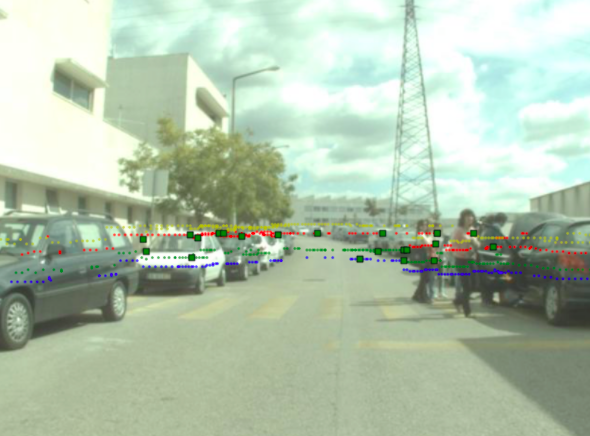
\includegraphics[height=2.8in, width=3.5in]{images/initial_result.png}
    \caption{ Initial segmentation results. Green squares are identified
    segments. Red, blue, yellow and green dots are Lidar points.}
  \end{figure}

  \subsection{Example Lidar Output}
  An example of the output of our system can be seen in Figure 1. Our lidar
  classifier does pick up the two woman on the right side of the image as two
  distinct pedestrians. There are additional people behind these two woman
  who are largely occluded and are not identified by our classifier. Unfortunately
  we also get several false positives around the cars on the left side of the road.

  \begin{figure}
    \includegraphics[height=2.8in, width=3.5in]{images/peopledetect.png}
    \caption{ Example output of OpenCV's peopledetect \cite{opencv}. }
  \end{figure}

  \subsection{Example OpenCV Output}
  An example of the output of OpenCV's peopledetect \cite{opencv} code can be seen in Figure 2.
  The results are surprisngly similar to our lidar classifier: it picks up the two
  women as well as two extra false positives. The output of OpenCV is more clearly
  indicated than the output of our lidar scans as they can draw very nice bounding
  boxes around the pedestrians. Unfortunately lidar scans do not provide any height
  information that can be extrapolated so estimated bounding boxes would have to be
  drawn with some assumption regarding the average height of a pedestrian.

%------------------------------------------------------------------------
\section{Future Work}
  As seen in Figure 1 and mentioned above, our lidar classfication does output a
  large number of false positives. While this is somewhat better than false negatives--
  identifying too many pedestrians is preferable over missing one--we believe that
  our results could be improved by minimizing false positives and more closely
  tying image classifications with our lidar classifications.

  \subsection{Minimizing False Positives}
  Since our lidar data consists of four horizontal scans taken at slightly different angles,
  we should expect that the existance of pedestrians results in several positive segment
  classifications (up to four) in the same area. Therefore, a simple way to decrease
  the number of positive classifications is to only positively classify segments if there
  are at least two other segment classifications in agreement within a small pixel margin.
  Taking Figure 1 for example, we get a large number of segments on the right side
  of the image around the two women which would be saved since there are many segments in
  agreement vertically. However, the other false positives would mostly be ignored
  since several are mostly isolated (although the white car does appear to have 3 segments
  in agreement as well).

  \subsection{Correlation with Image Data}
  Another addition that could improve our results is making a final prediction based
  on the results of both the lidar classification and image classification. A simple
  set intersection of the general areas where the positive lidar segments and OpenCV
  bounding boxes are in agreement could cut down on the extra classifications coming from
  both our lidar classifier as well as OpenCV's peopledetect. An example of a potential
  output of such a system can be seen in Figure 3.

  \begin{figure}
    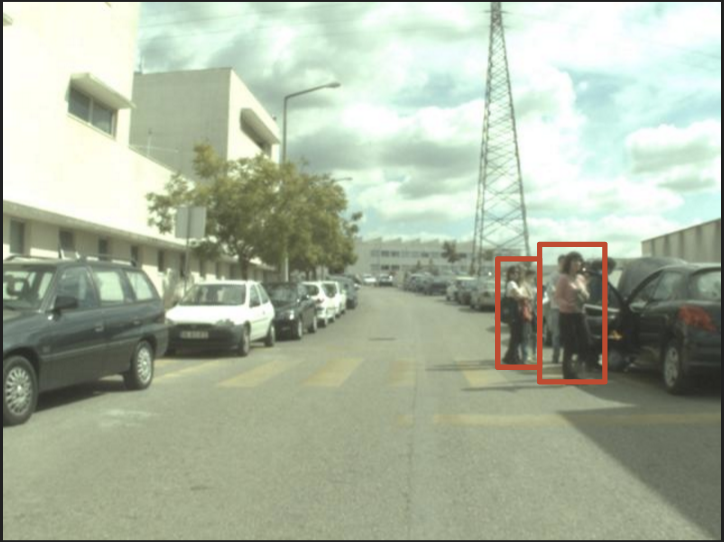
\includegraphics[height=2.8in, width=3.5in]{images/futureWork.png}
    \caption{ Example output of potential system that combines lidar with peopledetect.
    Bounding boxes are handdrawn. }
  \end{figure}

%------------------------------------------------------------------------
\section{Conclusion}
  We were able to successfully segment raw lidar scans, extract
  features, and make a classification. Unfortunately the final dataset that
  we test our system on provides labels as a series of bounding boxes on the
  image itself. As such, we did not have labels for individual segments and do
  not have an exact accuracy for our classifier. However, our intial examination
  of our results does look fairly positive: we generally do pick up pedestrians
  but also pick up other objects on the side of the road such as cars.

  Addition of the OpenCV peopledetect code provides additional interesting
  results. Similarly to our lidar classifier, OpenCV does generally detect
  pedestrians but also provides incorrect bounding boxes around cars and buildings.
  These incorrect classifications generally do not coincide with our lidar
  classifications and thereby validates our intial beliefs that a system combining
  both Lidar and Image classifications can perform better than either individually.

%------------------------------------------------------------------------

{\small
\bibliographystyle{ieee}
\bibliography{egbib}
}

\end{document}
